% Section content template for individual Educative lessons
% This file contains the actual content for a specific section
% Generated from Educative API section content

% Section: Use Case Diagram for the Vending Machine
% Section ID: 4732761898483712
% Section Slug: use-case-diagram-for-the-vending-machine
% Generated: 2025-12-11T20:25:39.470651

Let's build the use case diagram for the vending machine system and understand the relationships between its main actors and functions. First , we'll define the different elements of our system, followed by the complete use case diagram.

\subsection{System}\label{mp5h7PwOvSSW-z-hVU5e6}
\\
Our system is the vending machine. It manages automated product selection, payment, and goods dispensing through a self-service interface.

\subsection{Actors}\label{qJ2IsbfhPf2tTcj_ECpmY}
\\
Now, we'll define the main actors of our vending machine.

\subsubsection{Primary actors}\label{g466Vg-Wbx3lP0J--86x8}

\begin{itemize}
\item
\protect\phantomsection\label{ZngmkXn3uJ3ToILiz7xjx}
\textbf{Customer:} Can view available products, select products to purchase, insert money, collect dispensed products, and receive change.
\item
\protect\phantomsection\label{ipcZbF6rg_GVQH-rIDl99}
\textbf{Operator:} Inherits all customer actions. Additionally, the operator can add new products, remove products, and remove collected cash from the machine.
\end{itemize}

\subsection{Use cases}\label{vBJvd8FLO41o8l7DCLEfR}
\\
In this section, we will define the vending machine's use cases. We have listed them according to their respective interactions with a particular actor.

\subsubsection{Customer}\label{pzcuhXubNYl4iMGBAt3Oa}

\begin{itemize}
\item
\protect\phantomsection\label{9zljpZEUNwlsYhslAO7OQ}
\textbf{View products:} To view all available products in the vending machine.
\item
\protect\phantomsection\label{3zFATiSNfVLwcjhJWj-BH}
\textbf{Select product:} To select a product to buy by specifying the rack or slot number.
\item
\protect\phantomsection\label{JZl-83-GqKOmyIKvGsY_K}
\textbf{Insert money:} To insert cash to pay for the selected product.
\item
\protect\phantomsection\label{9ZDJkhkzU71X8TYQePgry}
\textbf{Take product:} To collect the dispensed product from the vending machine.
\item
\protect\phantomsection\label{RP5GgimjEYTFt_Qmcsq-4}
\textbf{Take change:} To collect change, if any, after the transaction.
\end{itemize}

\subsubsection{Operator}\label{GKDnjn107mYebMPUS2Lyl}
\\
Inherits all c\emph{ustomer} actions, plus:

\begin{itemize}
\item
\protect\phantomsection\label{NmMVBdRlR_0NuhJgpQKdG}
\textbf{Add product:} To add new products to the vending machine.
\item
\protect\phantomsection\label{SYjga_aI2gofHmprnMAAF}
\textbf{Remove product:} To remove products from the vending machine.
\item
\protect\phantomsection\label{UK6ho8zSTStfBgI_PAHVP}
\textbf{Remove cash:} To remove cash collected from the machine.
\end{itemize}

\subsubsection{System}\label{zg2nyepQ-leY24IMX_cFJ}

\begin{itemize}
\item
\protect\phantomsection\label{r50ZPYbnv-sb0yUMKzIyY}
\textbf{Search product:} To find and verify the selected product's availability in the machine.
\item
\protect\phantomsection\label{FJ5nqHH_Pw_i3xZusT_GC}
\textbf{Validate money:} To ensure the user has inserted enough money to buy the selected product.
\item
\protect\phantomsection\label{9YH2kxc5nTyCGEHsMi8ij}
\textbf{Dispense product:} To dispense the selected product to the user.
\item
\protect\phantomsection\label{apNXaDyjBuu-KNrLOJtf6}
\textbf{Return change:} To return change to the customer if the inserted amount exceeds the product price.
\end{itemize}

\subsection{Relationships}\label{te1-x8h8cdjBhzPmb1ax4}
\\
This section describes the relationships between and among actors and their use cases.

\subsubsection{Generalization}\label{O7_Nfljk0nlI5xF8gFFW3}
\\
The operator is a specialized role that extends the customer's capabilities (inherits all customer use cases, plus additional administrative ones).

\subsubsection{Associations}\label{UZ7I9fLU2J0SCZh69PRIv}
\\
The table below shows the association relationship between actors and their use cases.

\begin{center}
{\def\LTcaptype{none} % do not increment counter
\begin{longtable}[]{@{}
>{\raggedright\arraybackslash} p{(\linewidth - 4\tabcolsep) * \real{0.3333}}
>{\raggedright\arraybackslash} p{(\linewidth - 4\tabcolsep) * \real{0.3333}}
>{\raggedright\arraybackslash} p{(\linewidth - 4\tabcolsep) * \real{0.3333}}@{}}
\toprule\noalign{}
\endhead
\bottomrule\noalign{}
\endlastfoot
\begin{minipage}[t]{\linewidth}\raggedright
\textbf{Customer}
\end{minipage} & \begin{minipage}[t]{\linewidth}\raggedright
\textbf{Operator}
\end{minipage} & \begin{minipage}[t]{\linewidth}\raggedright
\textbf{System}
\end{minipage} \\
\begin{minipage}[t]{\linewidth}\raggedright
View products
\end{minipage} & \begin{minipage}[t]{\linewidth}\raggedright
Add product
\end{minipage} & \begin{minipage}[t]{\linewidth}\raggedright
Search product
\end{minipage} \\
\begin{minipage}[t]{\linewidth}\raggedright
Select product
\end{minipage} & \begin{minipage}[t]{\linewidth}\raggedright
Remove product
\end{minipage} & \begin{minipage}[t]{\linewidth}\raggedright
Dispense product
\end{minipage} \\
\begin{minipage}[t]{\linewidth}\raggedright
Insert money
\end{minipage} & \begin{minipage}[t]{\linewidth}\raggedright
Remove cash
\end{minipage} & \begin{minipage}[t]{\linewidth}\raggedright
Validate money
\end{minipage} \\
\begin{minipage}[t]{\linewidth}\raggedright
Take product
\end{minipage} & \begin{minipage}[t]{\linewidth}\raggedright
View product
\end{minipage} & \begin{minipage}[t]{\linewidth}\raggedright
Return change
\end{minipage} \\
\begin{minipage}[t]{\linewidth}\raggedright
Take change
\end{minipage} & \begin{minipage}[t]{\linewidth}\raggedright
Select product
\end{minipage} & \begin{minipage}[t]{\linewidth}\raggedright
\end{minipage} \\
\begin{minipage}[t]{\linewidth}\raggedright
\end{minipage} & \begin{minipage}[t]{\linewidth}\raggedright
Insert money
\end{minipage} & \begin{minipage}[t]{\linewidth}\raggedright
\end{minipage} \\
\begin{minipage}[t]{\linewidth}\raggedright
\end{minipage} & \begin{minipage}[t]{\linewidth}\raggedright
Take product
\end{minipage} & \begin{minipage}[t]{\linewidth}\raggedright
\end{minipage} \\
\begin{minipage}[t]{\linewidth}\raggedright
\end{minipage} & \begin{minipage}[t]{\linewidth}\raggedright
Take change
\end{minipage} & \begin{minipage}[t]{\linewidth}\raggedright
\end{minipage} \\
\end{longtable}
}
\end{center}

\subsubsection{Include}\label{E6c3ykAkGs3AZ07d6dOGz-2}
\\
In the use case diagram, ``include'' relationships show that one use case always incorporates the behavior of another. This helps clarify system workflows and makes the diagram modular and reusable.

\begin{itemize}
\item
\protect\phantomsection\label{PtTTrqta9nZ09MHXEORxh}
\textbf{Select product} → \textbf{Search product}

\begin{itemize}
\item
When a customer selects a product, the system must search for the selected product in its inventory to verify availability before proceeding.
\item
This ensures the product is in stock and ready for purchase.
\end{itemize}
\item
\protect\phantomsection\label{U3R-f-ic3C68hOrsqPGgk}
\textbf{Validate money} → \textbf{Dispense product}

\begin{itemize}
\item
After the customer inserts money and selects a product, the system must validate that the money is legal and sufficient for the purchase.
\item
Once validation succeeds, the ``Dispense product'' use case is included as the next step to physically provide the product to the customer.
\end{itemize}
\item
\protect\phantomsection\label{vOXKZ6EvnQxgXyRXXtEE0}
\textbf{Insert money} → \textbf{Validate money}

\begin{itemize}
\item
Once the customer inserts money to choose a product, the system checks whether the inserted amount is valid for purchasing the product. If it is, the customer proceeds to buy the product; otherwise, the system will ask the user to enter more money.
\end{itemize}
\item
\protect\phantomsection\label{x1CEaRCL492_aGQORd0NP}
\textbf{Validate money} → \textbf{Return change}

\begin{itemize}
\item
If the inserted amount is greater than the product price, after validating the money, the system must include the behavior of calculating and returning the correct change to the customer.
\end{itemize}
\end{itemize}

\subsection{Use case diagram}\label{CIpH3srIZCSszs9jPiB8J}
\\
Here's the use case diagram of the vending machine:

\begin{figure}[htbp]
 \centering
 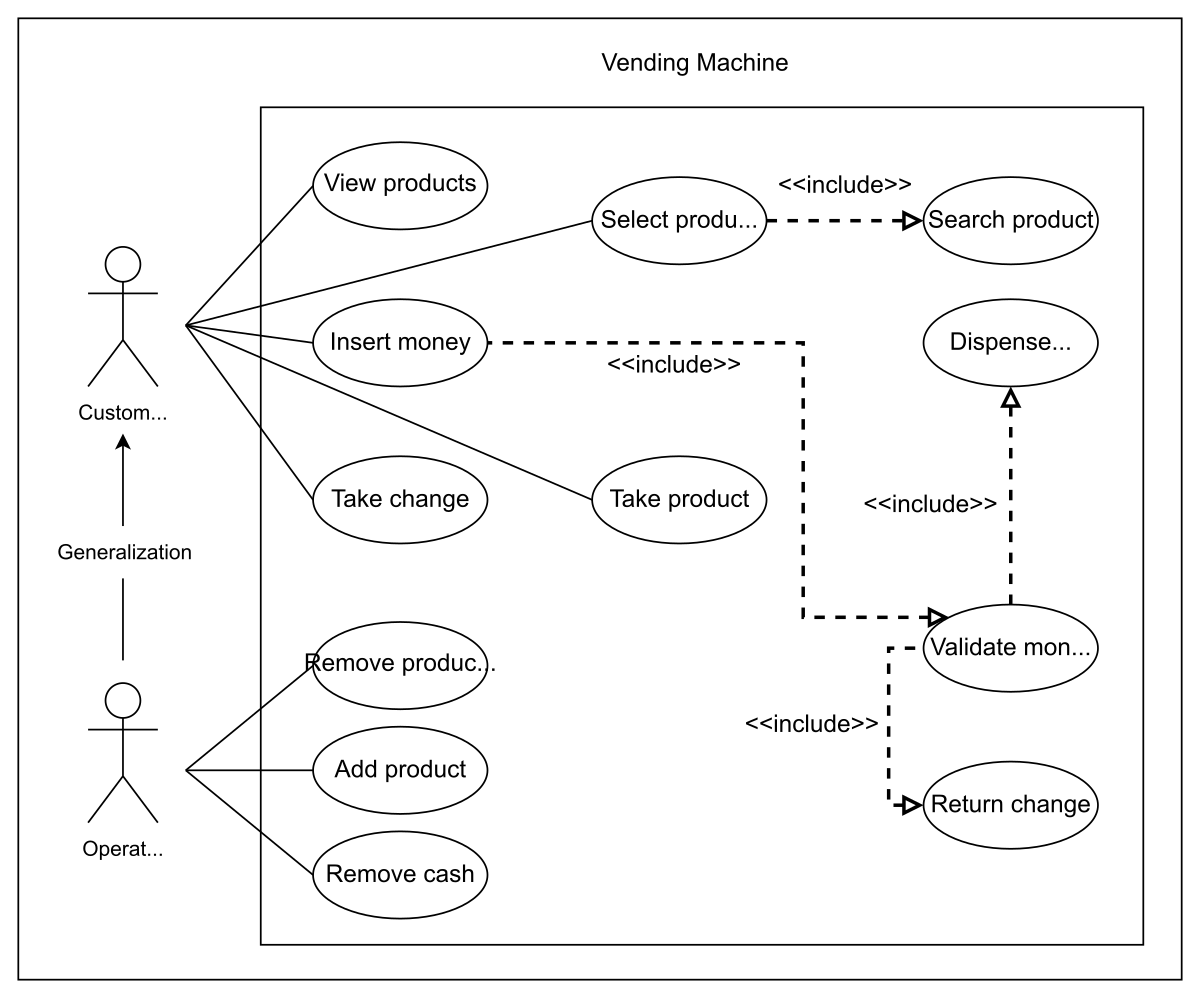
\includegraphics[width=0.5\textwidth]{Images/chapter_11/section_4732761898483712/4815330256748544.png}
 \caption{The use case diagram of the vending machine}
\end{figure}

In the next lesson, we'll discuss the class diagram with a detailed explanation of all classes and their relationship with each other.

% End of section content